
\documentclass[../main.tex]{subfiles}
\graphicspath{{\subfix{../images/}}}
\begin{document}
\textbf{....}
        \begin{figure}[bh]
        \centering
        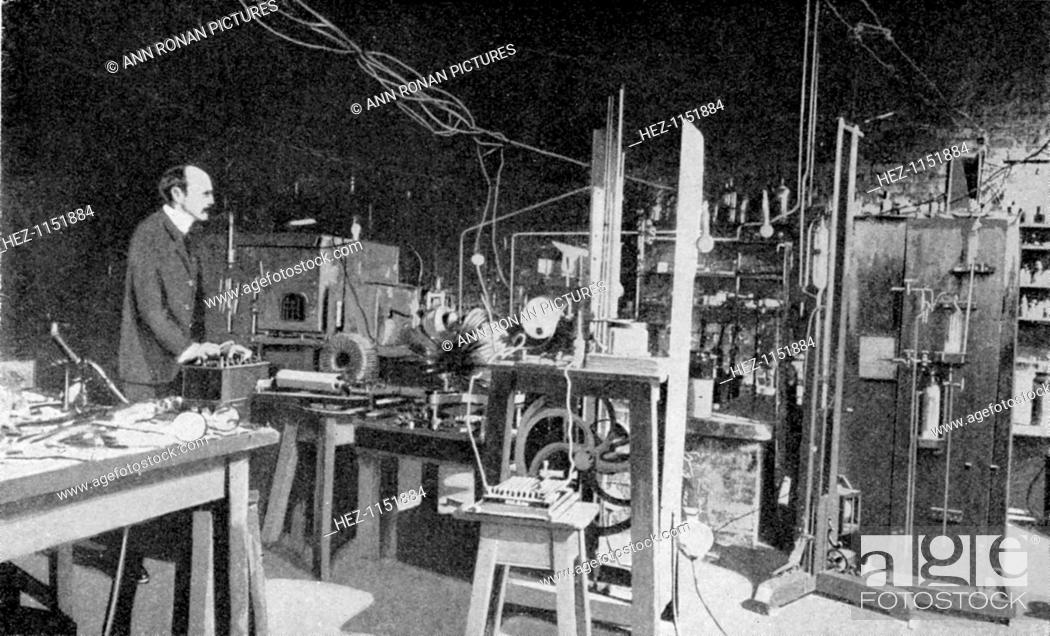
\includegraphics[width=3cm]{01.JJ-THOMSON-LAB}
        \label{fig:img1}
        \caption{JJ Thomson}
    \end{figure}
   
\begin{enumerate}[1. ] 
    \item \href{h https://www.youtube.com/watch?v=-Rb9guSEeVE&list=PLkyBCj4JhHt8DFH9QysGWm4h_DOxT93fb}{Electric Potential: Visualizing Voltage with 3D animations}
    \item \href{https://www.youtube.com/watch?v=f_MZNsEqyQw&list=PLkyBCj4JhHt8DFH9QysGWm4h_DOxT93fb&index=16}{Capacitors and Capacitance: Capacitor physics and circuit operation}
     \item \href{https://www.youtube.com/watch?v=P0Jnx1BjIZM&list=PLkyBCj4JhHt8DFH9QysGWm4h_DOxT93fb&index=29}{Electric Flux Paradox}
     \item \href{https://www.youtube.com/watch?v=eMTuPhg-8Go&t=22s}{Courant électrique : tension et intensité}
     \item \href{https://www.youtube.com/watch?v=m4jzgqZu-4s}{Electric Circuits: Basics of the voltage and current laws.}
     \item \href{https://www.youtube.com/watch?v=u4FpbaMW5sk}{Battery Energy and Power}
      \item \href{https://www.youtube.com/watch?v=5YYVnHN7xwM}{Charge to mass ratio of an electron}
      \item \href{https://www.youtube.com/watch?v=Ka3v5dIQGOI}{Crooke's Tube & Electrons}
       \item \href{https://fr.wikipedia.org/wiki/Bobine_Tesla}{Tesla Bobine COIL}
      \item \href{https://www.youtube.com/watch?v=QuLtuM8bAMI}{Demonstrating JJ Thomson experiment on charge to mass ratio}
      \item \href{https://www.youtube.com/watch?v=GR9A7Hd4mxQ}{JJ Thomson and the discovery of the electron}
      \item \href{https://www.youtube.com/watch?v=i6zyPOSreCg}{Cathode Ray Tube Experiment and Charge To Mass Ratio of an Electron}
    \item \href{https://www.youtube.com/watch?v=Rb6MguN0Uj4}{Discovery of the Electron: Cathode Ray Tube Experiment}

    \item \href{https://www.webassign.net/question_assets/unccolphyseml1/lab_4/manual.html}{Determination of e/m for the Electron}
    \item \href{https://physicsx.erau.edu/HelmholtzCoils/Lab_MP_1.pdf}{e/m ratio of the electron}
    \item \href{https://virtuelle-experimente.de/en/b-feld/e-m-bestimmung/edurchm.php}{Use the experiment to measure the ratio of the electrons charge to it's mass.}{}
    \item \href{https://www.physik.uzh.ch/~matthias/espace-assistant/manuals/en/anleitung_etom_e.pdf}{4. Electron Charge-to-Mass Ratio e/m - UZH - Physik-Institut}
    \item \href{https://demoweb.physics.ucla.edu/6b-lab-manual}{UCLA Physics \& Astronomy}
     \item \href{https://www.famousscientists.org/j-j-thomson/}{J. J. Thomson. Famous Scientists -The Art of Genius-}
     \item \href{https://virtuelle-experimente.de/en/index.php}{Electron Motion in Electric and Magnetic Fields}
\end{enumerate}

\textbf{Van Biezen - Magnetic fields and magnetic}
\begin{enumerate}[A.]
    \item \href{https://www.youtube.com/watch?v=kBoasyx8C_Y&list=PLX2gX-ftPVXX3FUB8FPKFPPXPJ6yhY4mT}{Physics - Magnetic Forces on Moving Charges - Direction (1 of 6) An Introduction}
    \item \href{https://www.youtube.com/watch?v=FXVJHjrgDuE&list=PLX2gX-ftPVXX3FUB8FPKFPPXPJ6yhY4mT&index=2}{Physics - Magnetic Forces on Moving Charges - Direction + Magnitude (2 of 6)}
    \item \href{https://www.youtube.com/watch?v=c6bcGfdLZ7c&list=PLX2gX-ftPVXX3FUB8FPKFPPXPJ6yhY4mT&index=3}{Physics - Magnetic Forces on Moving Charges - Direction + Magnitude (3 of 6)}
    \item \href{https://www.youtube.com/watch?v=DeAU6IQH0R4&list=PLX2gX-ftPVXX3FUB8FPKFPPXPJ6yhY4mT&index=4}{Physics - Magnetic Forces on Moving Charges - Direction + Magnitude (4 of 6)}
    \item \href{https://www.youtube.com/watch?v=qmzdN55zpTE&list=PLX2gX-ftPVXX3FUB8FPKFPPXPJ6yhY4mT&index=5}{Physics - Magnetic Forces on Moving Charges - Direction + Magnitude (5 of 6)}
    \item \href{https://www.youtube.com/watch?v=pw8seJUQ6VA&list=PLX2gX-ftPVXX3FUB8FPKFPPXPJ6yhY4mT&index=6}{Physics - Magnetic Forces on Moving Charges - Direction + Magnitude (6 of 6)}
    \item \href{https://www.youtube.com/watch?v=rCc5-IxUXEI&list=PLX2gX-ftPVXX3FUB8FPKFPPXPJ6yhY4mT&index=7}{Physics - E&M: Magn Field Effects on Moving Charge & Currents (7 of 26) F=? Current Loop}
    \item \href{https://www.youtube.com/watch?v=bc2sjL1wVDo&list=PLX2gX-ftPVXX3FUB8FPKFPPXPJ6yhY4mT&index=8}{Physics - E&M: Magn Field Effects on Moving Charge & Currents (8 of 26) Torque=? Current Loop}
    \item \href{https://www.youtube.com/watch?v=um_gDo3lUHs&list=PLX2gX-ftPVXX3FUB8FPKFPPXPJ6yhY4mT&index=9}{Physics - E&M: Magn Field Effects on Moving Charge & Currents (9 of 26) How Torque Changes}
    \item \href{https://www.youtube.com/watch?v=2Zi7ekMAZYU&list=PLX2gX-ftPVXX3FUB8FPKFPPXPJ6yhY4mT&index=10}{Physics - E&M: Magn Field Effects on Moving Charge & Currents (10 of 26) Magnetic Dipole Moment}
    \item \href{https://www.youtube.com/watch?v=urEBAiTr_-k&list=PLX2gX-ftPVXX3FUB8FPKFPPXPJ6yhY4mT&index=11}{Physics - E&M: Magn Field Effects on Moving Charge & Currents (11 of 26) P.E. of Magnetic Dipole}
    \item \href{https://www.youtube.com/watch?v=aqOY66dw1qU&list=PLX2gX-ftPVXX3FUB8FPKFPPXPJ6yhY4mT&index=12}{Physics - E&M: Magn Field Effects on Moving Charge & Currents (12 of 26) P.E.=? of Magnetic Dipole}
    \item \href{https://www.youtube.com/watch?v=fWaxrZHK5BY&list=PLX2gX-ftPVXX3FUB8FPKFPPXPJ6yhY4mT&index=13}{Physics - E&M: Magn Field Effects on Moving Charge & Currents (13 of 26) Force on a Current}
    \item \href{https://www.youtube.com/watch?v=UK4eBzmfsY0&list=PLX2gX-ftPVXX3FUB8FPKFPPXPJ6yhY4mT&index=14}{Physics - E&M: Magn Field Effects on Moving Charge & Currents (14 of 26) Force=? on a Current}
    \item \href{https://www.youtube.com/watch?v=YtN7_A8MeyE&list=PLX2gX-ftPVXX3FUB8FPKFPPXPJ6yhY4mT&index=15}{Physics - E&M: Magn Field Effects on Moving Charge & Currents (15 of 26) Torque=? Circular Current}
    \item \href{https://www.youtube.com/watch?v=DnHVgItjzu8&list=PLX2gX-ftPVXX3FUB8FPKFPPXPJ6yhY4mT&index=16}{Physics - E&M: Magn Field Effects on Moving Charge & Currents (16 of 26) The Velocity Selector}
    \item \href{https://www.youtube.com/watch?v=3fUjO2BoNFo&list=PLX2gX-ftPVXX3FUB8FPKFPPXPJ6yhY4mT&index=17}{Physics - E&M: Magn Field Effects on Moving Charge & Currents (17 of 26) Thompson's e/m Ratio}
    \item \href{https://www.youtube.com/watch?v=AR654M0Ruro}{Understanding Charge in magnetic field}
    \item \href{https://www.youtube.com/watch?v=fPST273JymU}{understanding charge in an electric field}
    \item \href{https://www.youtube.com/watch?v=vXOeehVTcRA}{Cathode Ray Tube | www.MyInterAcademy.com}
    \item \href{https://www.youtube.com/watch?v=8PRF-hrbAjk}{Class 9 Science - Structure of the Atom | Charged Particles in Matter}
     \item \href{https://www.youtube.com/watch?v=gTRVtDXMs4s}{From Geissler Tubes to Cathode Ray Tubes (Crookes Tubes), Physics & History}
\end{enumerate}
\textbf{Van Biezen - Physics 36 The Electric Fields}
\begin{enumerate}
    \item \href{https://www.youtube.com/watch?v=EPIhhbwbCNc&list=PLX2gX-ftPVXUcMGbk1A7UbNtgadPsK5BD&index=9}{Physics 36 The Electric Field (1 of 18)}
\end{enumerate}

\begin{enumerate}[1. ]
    \item \href{https://www.physicsread.com/latex-vector-bold/}{LATEX Physicsread}
    \item \href{https://physicsanduniverse.com/latex-symbols-and-using-them-to-write-equations/}{LaTeX Symbols and using them to write Equations}
    \item \href{https://texdoc.org/serve/siunitx/0}{siunitx – A comprehensive (SI) units package}
    \item \href{http://math.univ-lyon1.fr/irem/IMG/pdf/LatexPourLeProfDeMaths.pdf}{LATEX... pour le prof de maths }
\end{enumerate}
\end{document}


